\section{Quick Start}
\label{sec:cookbook}

\red{\textit{Cookbook-like description of pipeline recipes and their usage}}

\subsection{Important Concepts}
\subsubsection{The Trace-Wave Table}

\subsubsection{Detectors and Extensions}
Always use FITS extension names, not rely on the index/ordering.


\subsubsection{Pixels, Indices and Spectral Bins}
Pixel index starts at 1, not 0.

Also true when evaluating polynomials like race or wavecal.

Spectral bins correspond to detector columns at the mid-line of the extracted region (constant height).

Orders are indexed from 1..9, not always starting at 1, depending on cut-off orders. Index set by headers, conversion
to order number $m$ by XXX...

\subsubsection{Recipe naming conventions}
\begin{itemize}
    \item Cal
    \item Obs
    \item Util
\end{itemize}

\subsection{The Pipeline Recipes}
\label{sec:recipes-quick}

\red{\textit{Overview and/or summary of available pipeline recipes, i.e. list
    of available pipelines and a brief (one-liner) description of its purpose.}}

The naming convention groups the recipes into
\begin{itemize}
    \item \textit{Calibration recipes}, named like \texttt{cr2res\_cal\_*}
    \item \textit{Observing recipes}, named like \texttt{cr2res\_obs\_*}
    \item \textit{Utility recipes}, named like \texttt{cr2res\_util\_*}
\end{itemize}

\subsection{Data Formats}
\label{sec:data-fmt-quick}

\begin{figure}[!tb]
  \begin{center}
    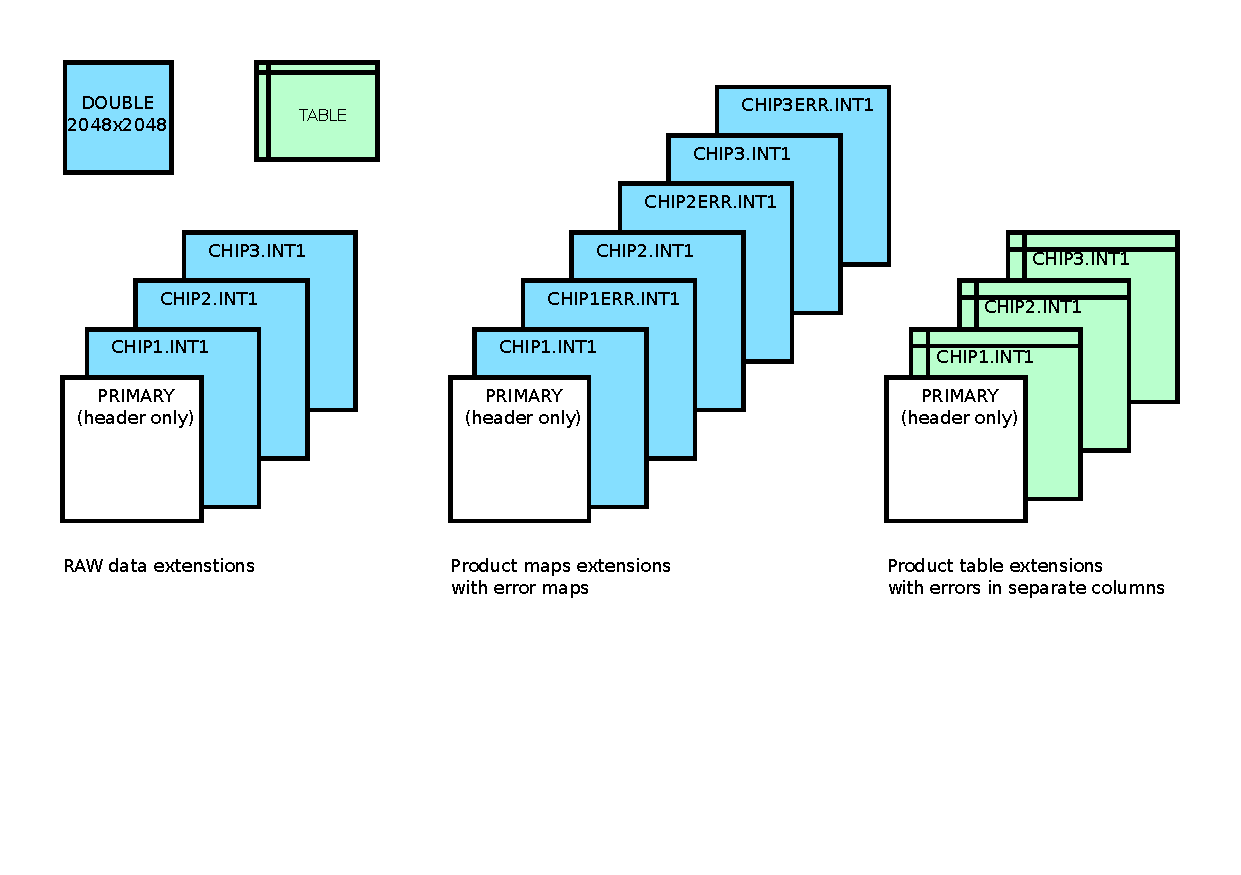
\includegraphics[width=0.99\linewidth]{fits_ext.pdf}
  \end{center}
  \caption{
    \label{fig:fits_ext}
    FITS extenstions in raw frames and data products.
    }
\end{figure}


\begin{figure}[!tb]
  \begin{center}
    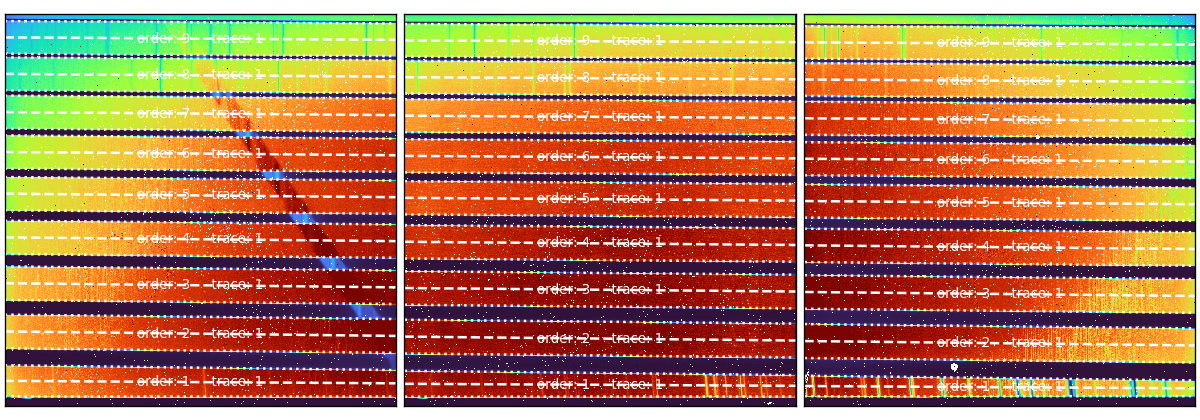
\includegraphics[width=0.99\linewidth]{J_2_3_03_cr2res_util_trace_out.png}
  \end{center}
  \caption{
    \label{fig:flat_trace}
    An example of a raw flat-field frame in J/2/3. Overplotted in white is 
    the result of the order tracing, the polynomial fit to the mid-line
    (dashed) and edges (dotted) for each detector-order.
    }
\end{figure}

trace-wave
image formats
BPM integers


The results of %TODO
are each stored as separate master calibration maps. Information about the orders 4,5,7 are stored together in a TW-table, as described in more detail %TODO ref.

\subsubsection{The Tracewave-Table}
\label{sec:tracewave}

table columns

polynomials, eval from 1 to 2048

meta-polynomials for slit curve.

\subsection{Executing Recipes}
\label{sec:exec-recipes-quick}


\subsubsection{Getting Started with \gasgano{}}
\label{sec:gasgano-quick}

\red{\textit{{Basic description of Gasgano and its usage with the \instrument{} and
  its recipes. Maybe omitted if Gasgano, for technical reasons cannot be
  supported (MUSE memory requirements for instance). If present, major parts
  will be provided by ESO.}}}

\subsubsection{Getting Started with \esorex{}}
\label{sec:esorex-quick}

\red{\textit{Basic description of \esorex{}. Contents will partially be
  provided by ESO, example follows.}}

\textit{\esorex{}} is a command-line tool which can be used to execute the
recipes of all standard VLT/VLTI instrument pipelines. With \textit{\esorex{}}
in your path, the general structure of an \textit{\esorex{}} 
command line is

\begin{shell}[fontsize=\small]
%prompt esorex [esorex options] [recipe [recipe options] [sof [sof]...]]
\end{shell}

where options appearing before the recipe name are options for
\textit{\esorex{}} itself, and options given after the recipe name are options
which affect the recipe. 

All available \textit{\esorex{}} options can be listed with the command
\begin{shell}[fontsize=\small]
%prompt esorex --help
\end{shell}

and the full list of available parameters of a specific recipe can be obtained
with the command 

\begin{shell}[fontsize=\small]
%prompt esorex --help <recipe name>
\end{shell}
The output of this command shows as parameter values the current setting, \ie
all modifications from a configuration file or the command line are already
applied.

The listing of all recipes known to \textit{\esorex{}} can be obtained with the command
\begin{shell}[fontsize=\small]
%prompt esorex --recipes
\end{shell}

The last arguments of an \textit{\esorex{}} command are the so-called
\textit{set-of-frames}. A \textit{set-of-frames} is a simple text file which
contains a list of input data files for the recipe. Each input file is
followed by an unique identifier (frame classification or frame tag),
indicating the contents of this file. The input files have to be given as an
absolute path, however \textit{\esorex{}} allows the use of environment variables so
that a common directory prefix can be abreviated. Individual lines may be
commented out by putting the hash character (\texttt{\#}) in the first
column. An example of a \textit{set-of-frames} is shown in the following:

\begin{shell}[fontsize=\small]
%prompt cat bias.sof
/data/cr2res/raw/CR2RES.2019-03-29T09:48:53.153.fits BIAS
$RAW_DATA/CR2RES.2019-03-29T09:50:36.645.fits BIAS
$RAW_DATA/CR2RES.2019-03-29T09:52:16.513.fits BIAS
$RAW_DATA/CR2RES.2019-03-29T09:53:47.996.fits BIAS
#$RAW_DATA/CR2RES.2019-03-29T09:55:04.515.fits BIAS
\end{shell}

These \textit{set-of-frames} files will have to be created by the user using a
text editor, for instance. Which classification has to be used with which
recipe will be shown in section \ref{sec:dataorganization}

Finally, if more than one \textit{set-of-frames} is given on the command-line \textit{\esorex{}}
concatenates them into a single \textit{set-of-frames}.

\subsection{Data Organization}
\label{sec:dataorganization}

\red{\textit{Outline of how to organize \instrument{} data, i.e. how to get to
    a correct SOF file, which classification tags are accepted by the recipes
    and how they are defined in terms of header keywords.}}
